\documentclass[11pt]{ltjsarticle}
\usepackage{amsmath}
\usepackage{amssymb}
\usepackage{amsfonts}
\usepackage{physics}
\usepackage{graphicx}
\usepackage{float}
\usepackage{booktabs}
\usepackage{tikz}
\usepackage{xcolor}
\usepackage{pgfplots}
\usepackage{mathcomp}
\usepackage{enumitem}
\usepackage{wrapfig}
\usepackage{etoolbox}
\usepackage{cleveref}
\usepackage[version=4]{mhchem}
\crefformat{figure}{図~#2#1#3}  % 図の日本語設定
\crefformat{equation}{式~(#2#1#3)}  % 式の日本語設定
\crefformat{table}{表~#2#1#3}  % 表の日本語設定
\usetikzlibrary{intersections,calc}
\pgfplotsset{compat=1.18}
\begin{document}
\begin{figure}[H]
  \centering
  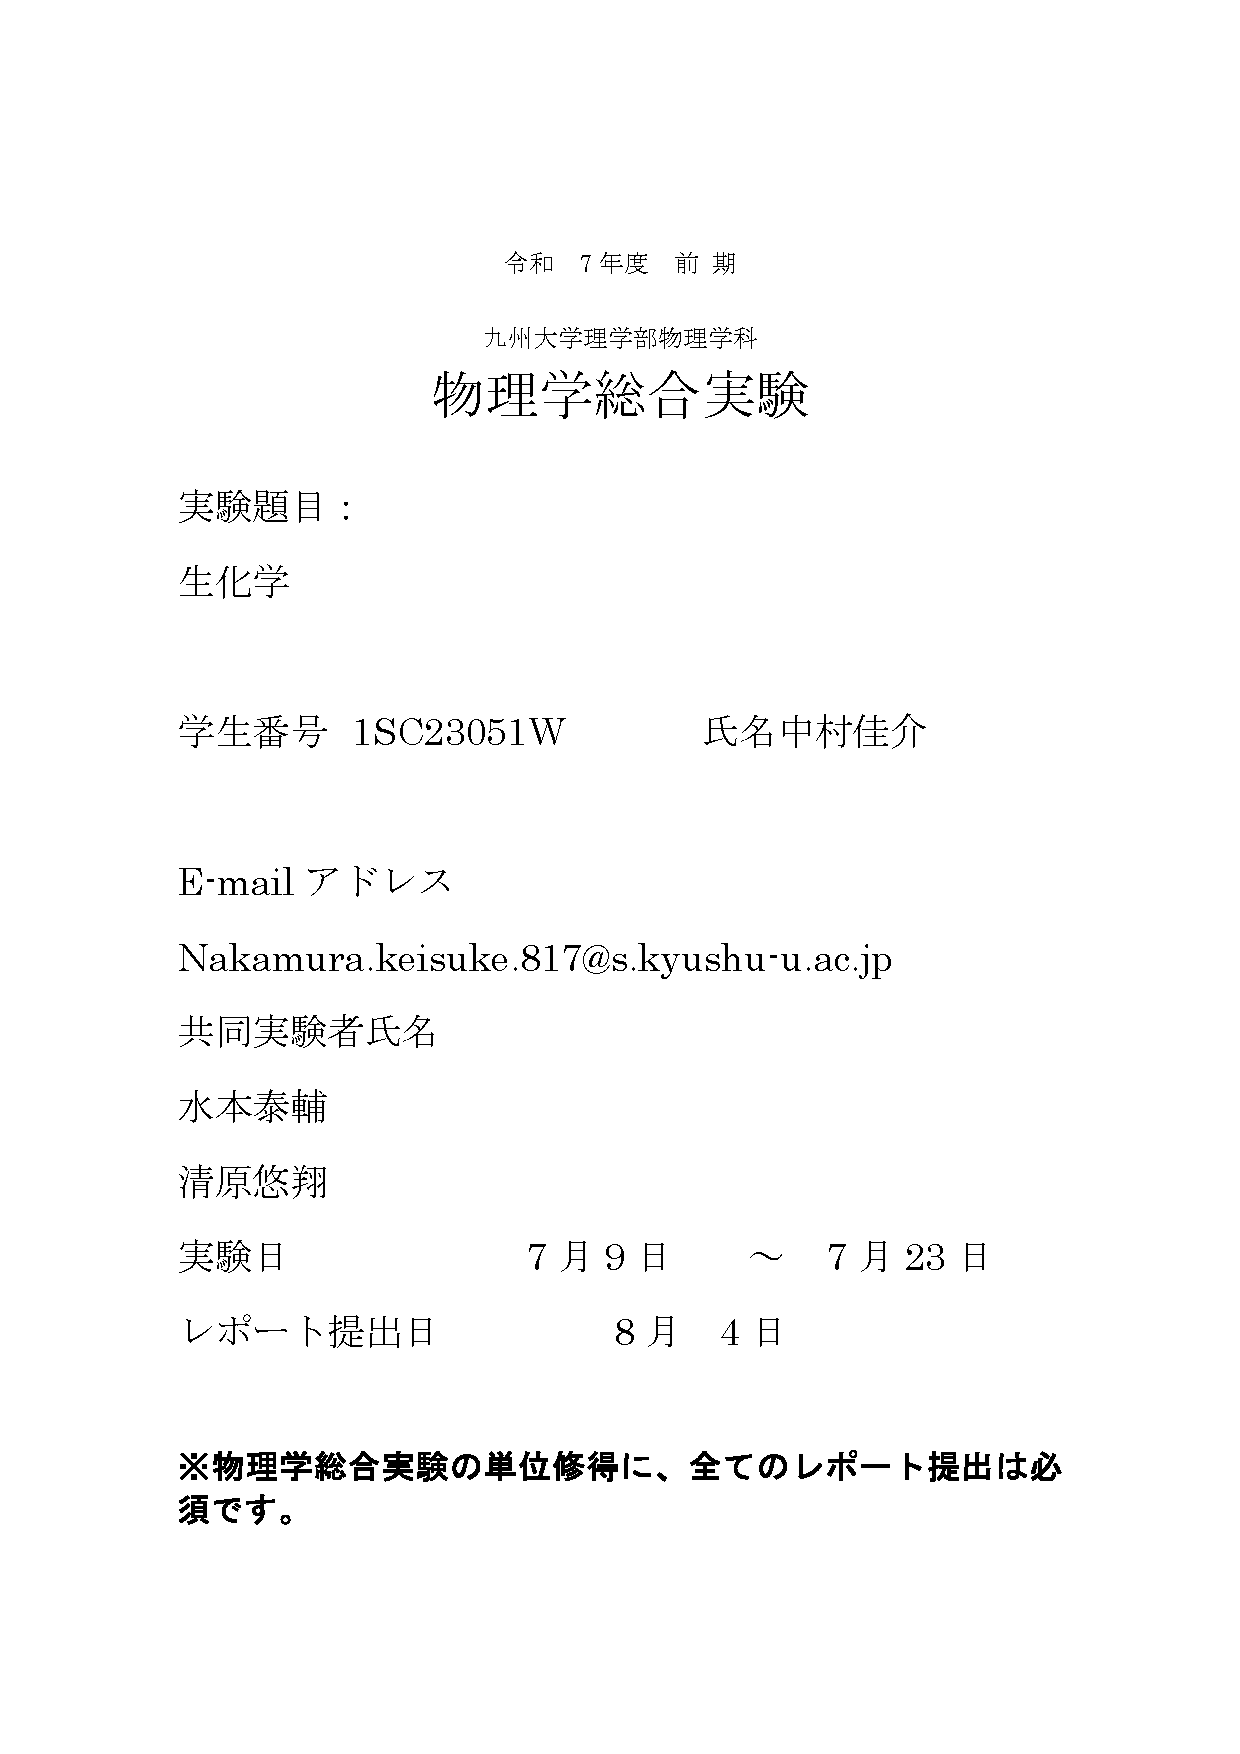
\includegraphics[width=\textwidth]{hyoushi.pdf}
\end{figure}
  \section*{目的}
    \begin{enumerate}
      \item 微粒子のブラウン運動から, 分子の存在を確認する.
      \item ブラウン運動の統計的な解析手法について学ぶ.
      \item 原子よりもはるかに大きいが, 目に見える大きさよりはるかに小さいメソ(中間的)スケールの粒子が大きな役割を果たす生体物質の物性や統計的性質について学ぶ.
      \item 現在の研究に不可欠なPCを用いた測定, 解析手法について学ぶ.
    \end{enumerate}
  \section*{原理}
    \subsection*{ブラウン運動}
      ブラウン運動は, 液体や気体中に浮遊する微粒子が不規則に運動する現象であり, 1827年にロバート・ブラウンによって発見された. ブラウン運動の本質は, 微粒子が周囲の分子から受けるランダムな衝突によって生じる. この衝突は分子の熱運動に起因し, 微粒子は連続的かつ予測不可能な軌道を描く.\\
      この現象は, 分子の存在を直接的に示す重要な証拠となり, 統計力学や拡散現象の理解に不可欠である. アインシュタインは1905年に, ブラウン運動を理論的に説明し, 拡散係数$D$と平均二乗変位$\langle x^2 \rangle$の関係を導出した:
      \begin{equation}
        \langle x^2 \rangle = 2 D t, D = \frac{R T}{6 \pi \eta a N_A}
        \label{eq:einstein}
      \end{equation}
      ここで$D$は拡散係数, $t$は時間, $R$は気体定数, $T$は絶対温度, $\eta$は媒質の粘性係数, $a$は粒子の半径である.
      ここで$N_A$以外の値は実験的に測定可能であり, 原子の性質を一切考えることなくアボガドロ数$N_A$を求めることができる.
      \cref{eq:einstein}の式は, 一次元運動のときであるが, 次元が増えても各方向の運動が独立ならば単純に足すことができる. したがって, 二次元の場合は以下の式になる.
      \begin{equation}
        \langle x^2 + y^2 \rangle = 4 D t
        \label{eq:einstein_2d}
      \end{equation}
      実験的には, 顕微鏡下で微粒子の位置を時間ごとに記録し, その軌跡から平均二乗変位を算出することで, アボガドロ数を求めることができる.
      \newpage
    \subsection*{生体物質の挙動}
      \begin{wrapfigure}{r}{0.4\textwidth}
        \centering
        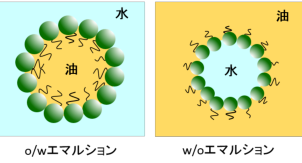
\includegraphics[width=0.38\textwidth]{emal.png}
      \end{wrapfigure}
      生体物質は, タンパク質やDNA, 細胞内器官, 赤血球など, メソスケール(数10 nm~10 µm)の構造を持つものが多い.
      これらの構造は, 物性や機能に大きな影響を与えている.
      例えば, 牛乳は水(乳清)中にタンパク質で安定化された脂肪液滴が分散したエマルション(乳濁液)であり, この微細な脂肪球が光を散乱することで白く見える.
      今回, 実験では脂肪球の様子を観察し, 酸などの刺激に応じてエマルション状態が変化する様子を観察する.
      \subsubsection*{壁面効果}
      壁面近傍では、粒子が壁と平行に移動する際の粘性抵抗が増加する.抵抗係数$\gamma_\parallel$は, 壁と粒子重心間の距離$z$を用いて次式で近似される.
      \begin{equation}
        \gamma_\parallel = \left[ 1 - \frac{8}{15} \ln \left( 1 - \frac{a}{z} \right) \right] \gamma
        \label{eq:wall_effect}
      \end{equation}
  \section*{実験方法}
    \subsection*{実験器具}
    \begin{minipage}{0.58\columnwidth}
      \cref{fig:setup}のような装置を用いて, 微粒子のブラウン運動を観察する.
      \subsubsection*{顕微鏡の扱い方}
        \begin{itemize}
          \item レンズや光学系には触れず、ステージ昇降ハンドルで高さ調整する.
          \item 焦点合わせは低倍率レンズで行い、徐々に高倍率へ切り替え.
          \item USBカメラ接続後, PCソフトで画像を調整・保存する.
          \item 観察中は振動や衝撃を与えない.
        \end{itemize}
    \end{minipage}
      \begin{minipage}{0.38\textwidth}
        \begin{figure}[H]
          \centering
          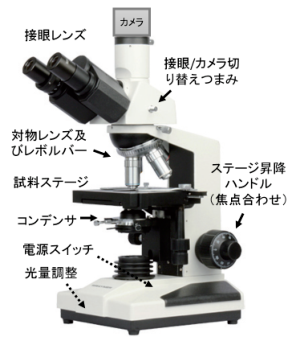
\includegraphics[width=\textwidth]{kigu.png}
          \caption{実験装置の概略図}
          \label{fig:setup}
        \end{figure}
      \end{minipage}
        \newpage
    \subsection*{試料作製}
      \subsubsection*{ポリスチレン粒子の調製}
      \begin{enumerate}
        \item 直径2µmのポリスチレン粒子が入った体積分率2.5\%の原液を1000倍希釈した.
        \item スライドガラスにシリコンゴムリングを置き, その中に20µLの希釈液を滴下し、カバーガラスをかぶせた.
      \end{enumerate}
    \subsubsection*{脂肪球}
      \begin{enumerate}
        \item 牛乳を100倍希釈したのち, さらに10倍希釈した. 
        \item スライドガラスにシリコンゴムはおかず, 20µLの希釈液を滴下し, カバーガラスをかぶせた.
        \item 酸による変化を観察するため, 酢酸の20v\%水溶液1mlを用意した.
        \item 溶液を希釈し, 10,2,0,2v\%の濃度にしたものをそれぞれ0.5ml用意した. 酢酸20\%水溶液, 水もそれぞれ0.5ml用意した.
        \item 各チューブに同体積の牛乳を加え, 手で振って混合したのちに10分間静置した. 
        \item 各チューブから少量をスライドガラスに滴下し, カバーガラスをかぶせた.
      \end{enumerate}
    \subsection*{測定手順}
      \subsubsection*{ポリスチレン粒子}
        \begin{enumerate}
          \item 1粒子の運動を解析し, 軌跡と速さのデータから見えている運動がブラウン運動であることを確認した.
          \item 4粒子の軌跡データからそれぞれ平均二乗変位(MSD)を求め, アボガドロ数を求めた.
          \item 直径3µm,直径1µmのポリスチレン粒子を用意し, 同様の手順で測定した.
        \end{enumerate}
      \subsubsection*{脂肪球}
        \begin{enumerate}
          \item 脂肪球の運動からMSDを求め, 脂肪球の大きさを計算し, 画像から求めた大きさと比較した.
          \item 脂肪球の浮上速度を測定した.
          \item 酢酸の濃度によって脂肪球のエマルション状態がどのように変化するかを観察した.
        \end{enumerate}
  \section*{結果}
    \subsection*{課題1}
      2\mu mのポリスチレン粒子のブラウン運動の軌跡を観察した結果, 以下のような軌跡,速度分布が得られた.\\
      \begin{minipage}{0.48\textwidth}
        \begin{figure}[H]
          \centering
          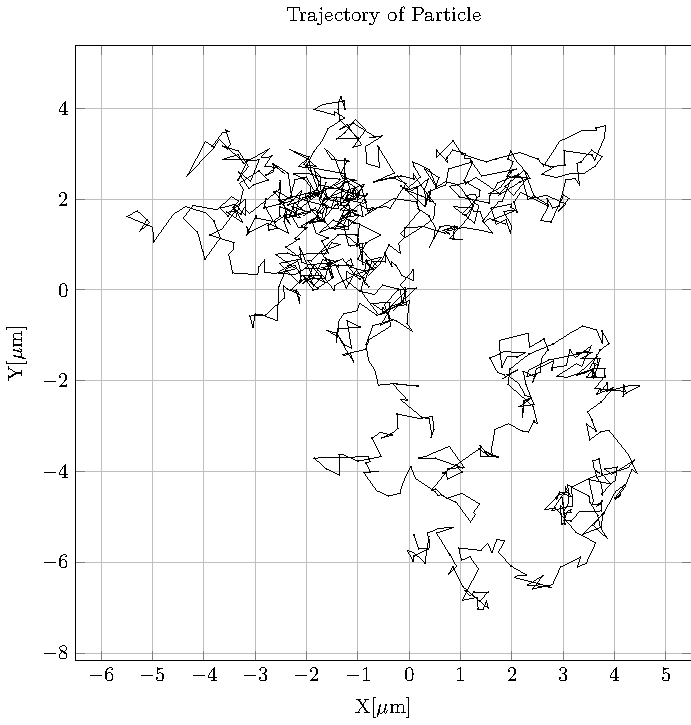
\includegraphics[width=\linewidth]{graph2u_1.pdf}
          \caption{2µmポリスチレン粒子のブラウン運動の軌跡(重心まわり)}
          \label{fig:2ps_track1}
        \end{figure}
      \end{minipage}
      \hfill
      \begin{minipage}{0.48\textwidth}
        \begin{figure}[H]
          \centering
          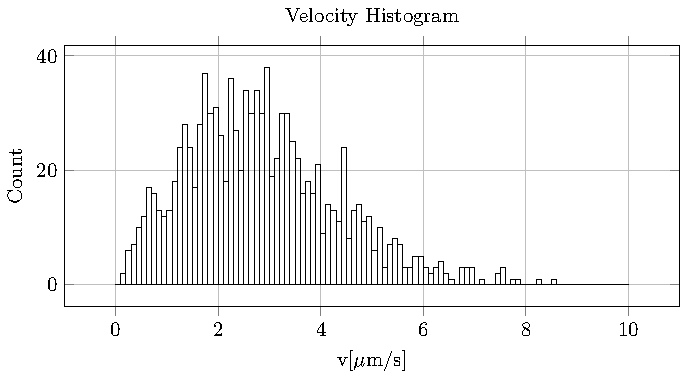
\includegraphics[width=\linewidth]{graph2uv_1.pdf}
          \caption{2µmポリスチレン粒子のブラウン運動の速度分布}
          \label{fig:2ps_speed1}
        \end{figure}
      \end{minipage}
      \\
      これらのグラフを見ると, 粒子の運動はランダムで, 速度はばらばらであり, ブラウン運動であることがわかる.
    \subsection*{課題2}
      2\mu mのポリエチレン粒子のブラウン運動の軌跡を4粒子について観察した結果, 以下のような軌跡,速度分布が得られた.\\
      \begin{minipage}{0.48\textwidth}
        \begin{figure}[H]
          \centering
          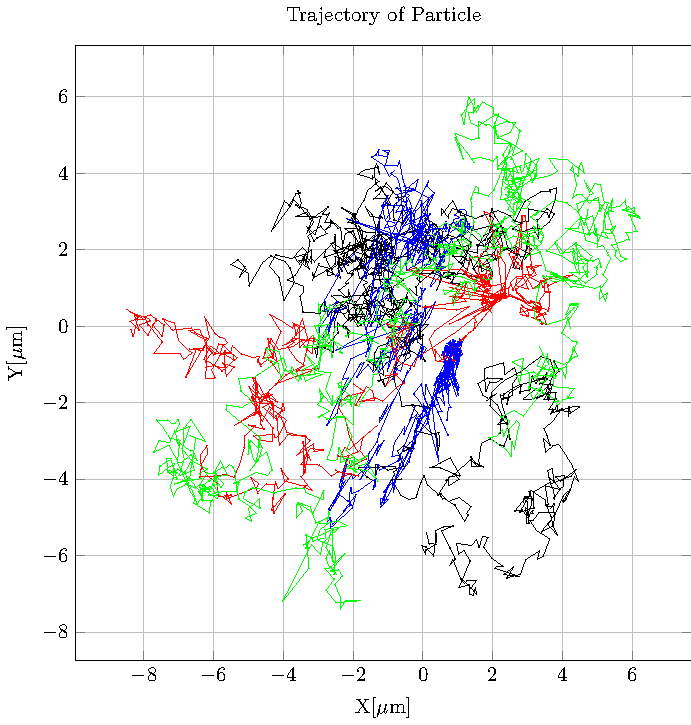
\includegraphics[width=\linewidth]{graph2u.pdf}
          \caption{2µmポリスチレン4粒子のブラウン運動の軌跡(重心まわり)}
          \label{fig:2ps_track}
        \end{figure}
      \end{minipage}
      \hfill
      \begin{minipage}{0.48\textwidth}
        \begin{figure}[H]
          \centering
          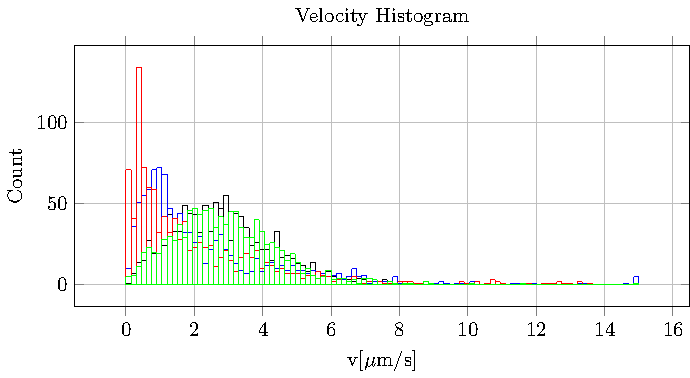
\includegraphics[width=\linewidth]{graph2uv.pdf}
          \caption{2µmポリスチレン4粒子のブラウン運動の速度分布}
          \label{fig:2ps_speed}
        \end{figure}
      \end{minipage}
      \\
      これらのグラフを見ると, 赤色の粒子以外はランダムな軌跡, 同様の速度分布を示しているが, 赤色の粒子は特定の位置に留まっており, その影響で小さい速度の分布が大きくなっていることがわかる.\\
      こうなった要因として, 粒子間の衝突や, 粒子が壁に近づきすぎていることが考えられる. 
      同様に, 直径3µm,1µmのポリスチレン粒子についても同様の測定を行い, 以下のような結果が得られた.\\
      \begin{minipage}{0.48\textwidth}
        \begin{figure}[H]
          \centering
          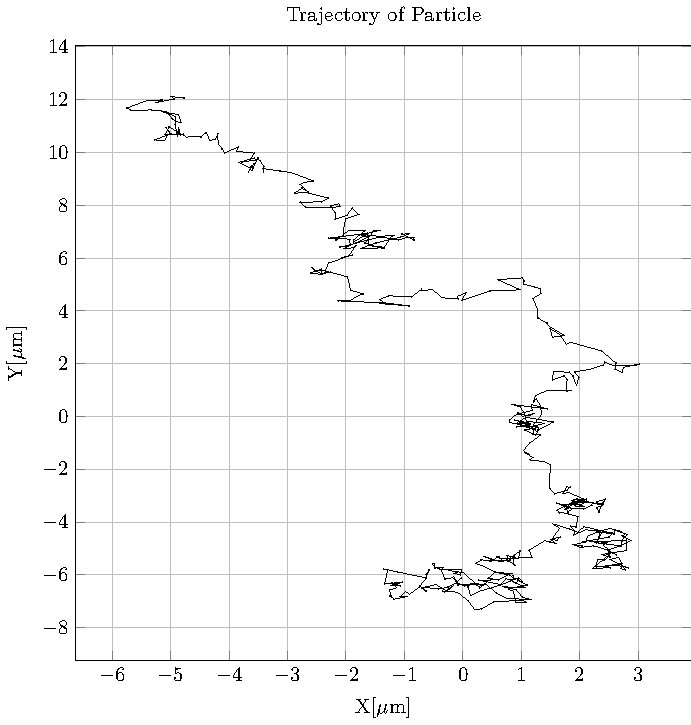
\includegraphics[width=\linewidth]{graph3u.pdf}
          \caption{3µmポリスチレン粒子のブラウン運動の軌跡(重心まわり)}
          \label{fig:3ps_track}
        \end{figure}
      \end{minipage}
      \hfill
      \begin{minipage}{0.48\textwidth}
        \begin{figure}[H]
          \centering
          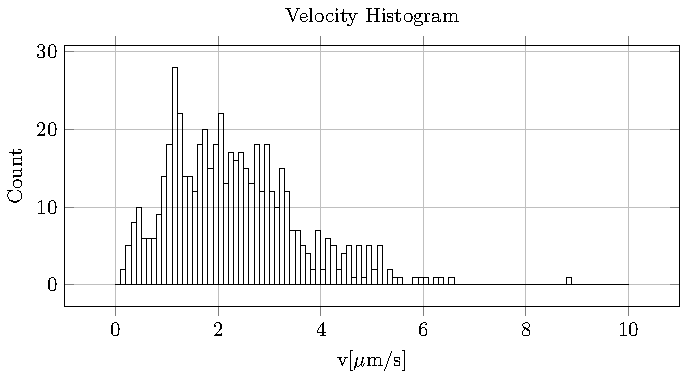
\includegraphics[width=\linewidth]{graph3uv.pdf}
          \caption{3µmポリスチレン粒子のブラウン運動の速度分布}
          \label{fig:3ps_speed}
        \end{figure}
      \end{minipage}
      \\
      \begin{minipage}{0.48\textwidth}
        \begin{figure}[H]
          \centering
          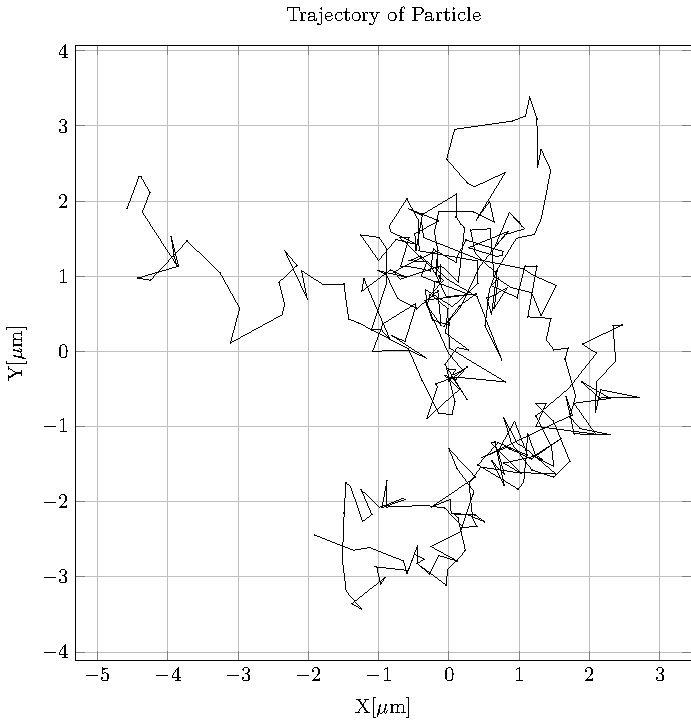
\includegraphics[width=\linewidth]{graph1u.pdf}
          \caption{1µmポリスチレン粒子のブラウン運動の軌跡(重心まわり)}
          \label{fig:1ps_track}
        \end{figure}
      \end{minipage}
      \hfill
      \begin{minipage}{0.48\textwidth}
        \begin{figure}[H]
          \centering
          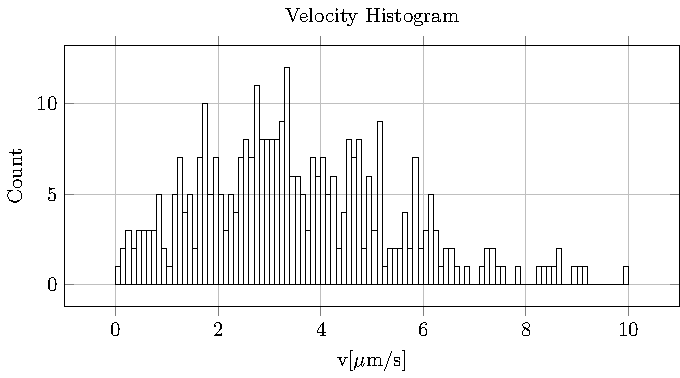
\includegraphics[width=\linewidth]{graph1uv.pdf}
          \caption{1µmポリスチレン粒子のブラウン運動の速度分布}
          \label{fig:1ps_speed}
        \end{figure}
      \end{minipage}
      これらを見ると, 直径3µmの粒子はブラウン運動以外の運動をしているような挙動が見られた. また, 直径1µmの粒子は, 直径2µmの粒子と同様にランダムな軌跡を示しているが, 速度分布はボリュームゾーンが右にずれたことがわかる.\\
    \subsection*{発展課題:沈降速度と沈降平衡}
      ある粒子に働く重力と浮力, 抵抗力の釣り合いを考える.
      \begin{equation}
        mg = \rho V g + 6 \pi \eta a v
        \label{eq:stokes}
      \end{equation}
      ここで$m$は粒子の質量, $\rho$は媒質の密度, $V$は粒子の体積, $g$は重力加速度, $\eta$は媒質の粘性係数, $a$は粒子の半径, $v$は沈降速度である.
      ここに, a=1µm, $\rho=1.0 \mathrm{g/cm^3}$, $\eta=0.890 \mathrm{mPa\cdot s}$とすると,
      v=0.245µm/sとなる.\\
      また, 粒子間相互作用がない理想形と考えると, 十分に時間がたった時の垂直方向の密度分布は異なるポテンシャルにある粒子の分布と考えられる.
      したがってその分布は, ボルツマン分布にしたがい,
      \begin{equation}
        n(h)= n_0 \exp\left(-\frac{U(h)}{kT}\right) = n_0 \exp\left(-\frac{(\rho-\rho_{aqua})gh}{kT}\right)
        \label{eq:boltzmann}
      \end{equation}
      となる. ここで$h$は粒子の高さ, $n(h)$は高さ$h$における粒子の密度, $n_0$は基準密度, $U(h)$は高さ$h$におけるポテンシャルエネルギー, $k$はボルツマン定数, $\rho_{aqua}$は水の密度, $\rho$は粒子の密度である.
    \subsection*{発展課題:緩和時間}
      緩和時間を計算すると, \tau = $2.74 \times 10^{-7}$ sとなる. このことから, 計算した速度は高々0.1sの間の速さであり, ブラウン運動そのものの速度ではない. 
    \subsection*{課題3}
      直径2\mu mのmsdを求めた結果, 以下のようなグラフが得られた.\\
      \begin{figure}[H]
        \centering
        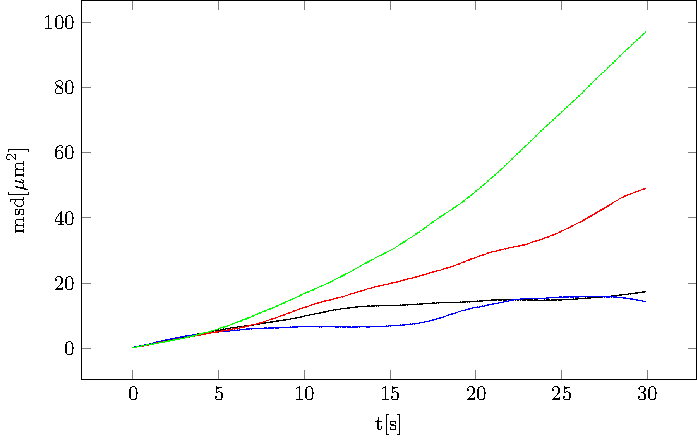
\includegraphics[width=0.6\linewidth]{graph2u_msd.pdf}
        \caption{2µmポリスチレン粒子のMSD}
        \label{fig:2ps_msd}
      \end{figure}
    これを見ると, 各粒子のMSD0-5sではほぼ同じで, それ以降ずれていっていることがわかる.
    このように, tが大きくなるにつれ, msdがずれていくのは, ブラウン運動というランダムな運動に対して, ある方向への運動(溶液の流れなど)が加わることによって, 長い時間でみると, その方向への運動が大きくなるためである.\\
    また, 統計的には時間差$\delta t$が小さくなると, サンプル数が増えるので, 大数の法則により, MSDの値は理論に近づく.
    \subsection*{課題4}
      各粒子の0-5s間のMSDからアボガドロ数を求めた結果, 以下のような値が得られた.\\
      粒子1: $\mathrm{N_A} = 4.66 \times 10^{23} \mathrm{mol^{-1}}$,
      粒子2: $\mathrm{N_A} = 4.73 \times 10^{23} \mathrm{mol^{-1}}$,\\
      粒子3: $\mathrm{N_A} = 5.09 \times 10^{23} \mathrm{mol^{-1}}$,
      粒子4: $\mathrm{N_A} = 4.78 \times 10^{23} \mathrm{mol^{-1}}$\\
      これらの値から, この実験でのアボガドロ数は
      $\mathrm{N_A} = 4.815\pm0.0821 \times 10^{23} \mathrm{mol^{-1}}$となった.
    \subsection*{発展課題:ほかの手法}
      ほかの手法として, 
      \begin{itemize}
        \item ファラデー定数と素電荷の比から求める方法
        \item 陽子の核磁気回転などから求める方法
        \item X線回折と結晶の密度から求める方法
        \item 単結晶の格子定数を精密に求める方法
      \end{itemize}
      などがある. 現在, アボガドロ数は定義値である. この定義値は最後の方法によって, 不純物, 欠陥が少ない単結晶シリコンを用いて定義された.
    \subsection*{発展課題:マイクロレオロジー}
      マイクロレオロジーは, 細胞内部の物性測定, コラーゲンなどの高分子が溶液からゲルに変化する過程の測定などに用いられている.
    \subsection*{課題5}
      3粒子の0-5s間のMSDから粒子の半径を求めた結果と画像から半径を求めたところ,  以下のような値が得られた.\\
      \begin{table}[H]
        \centering
        \begin{tabular}{|c|c|c|}\hline
          粒子 & MSDから求めた半径[µm] & 画像から求めた半径[µm] \\
          \hline
          粒子1 & 3.20 & 3.26 \\\hline
          粒子2 & 4.47 & 5.63\\\hline
          粒子3 & 5.83 & * \\\hline
        \end{tabular}
        \caption{脂肪球の半径}
        \label{tab:ps_radius}
      \end{table}
      粒子3についてはデータ不備で画像から半径を求めることができなかった.
      粒子1,2については, MSDから求めた値と画像から求めた値はほぼ一致していることがわかる.\\
    \subsection*{課題6}
      脂肪球の浮上速度は1.0\mu mであった. 浮上速度が速く, セル中央部での軌跡を得ることはできなかった. 
    \subsection*{課題7}
      酢酸の濃度による脂肪球のエマルション状態の変化を観察した結果, 以下のような画像が得られた.\\
      \begin{figure}[H]
        \centering
        \begin{minipage}{0.48\textwidth}
          \centering
          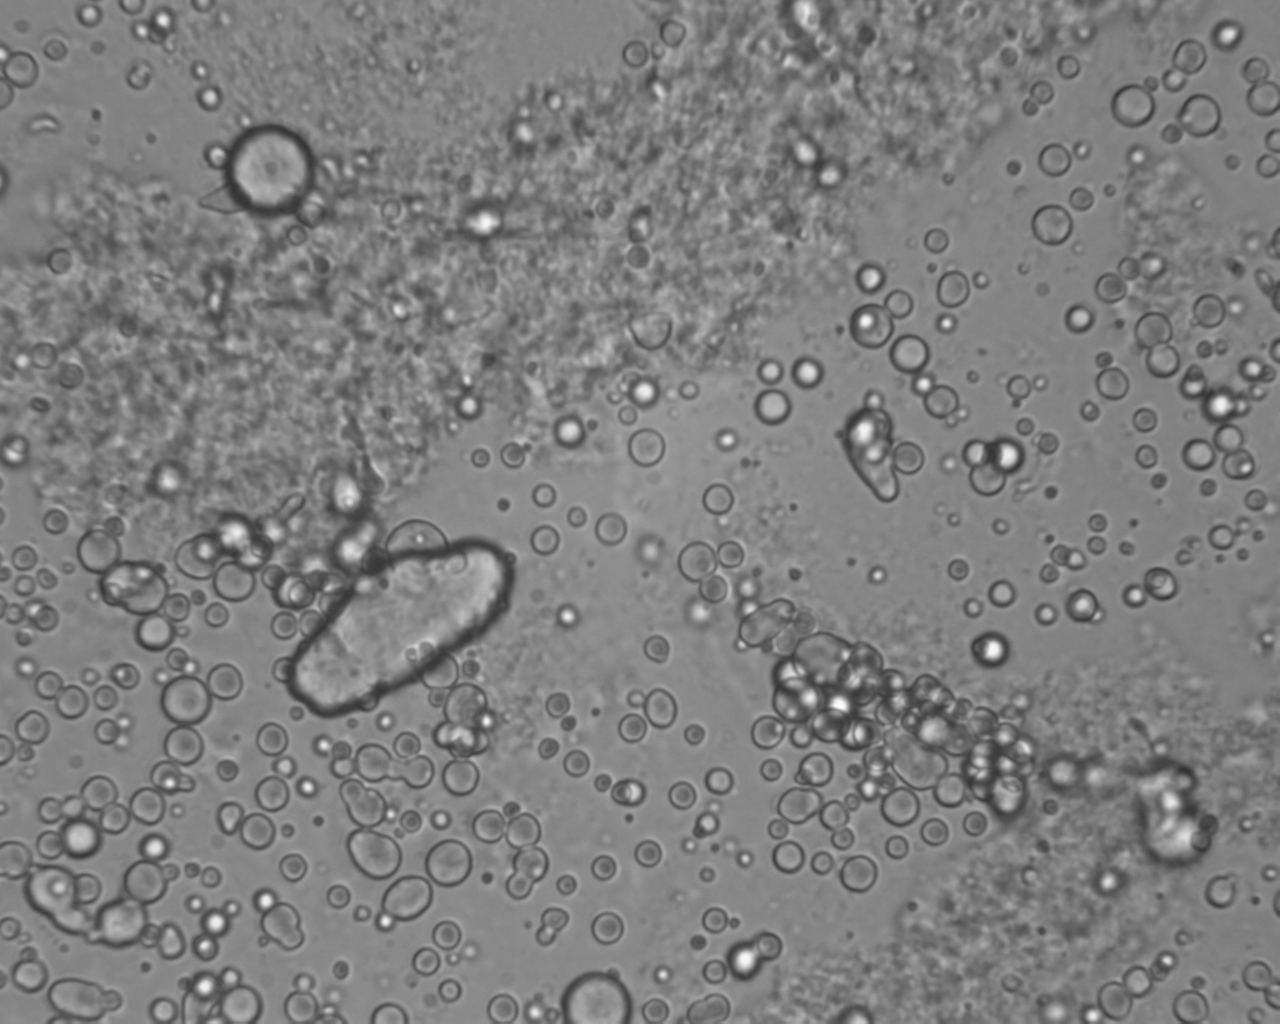
\includegraphics[width=\linewidth]{mizumoto_0.2_1.png}
          \caption{0.2v\%酢酸添加後の脂肪球1}
          \label{fig:milk0.2_1}
        \end{minipage}
        \hfill
        \begin{minipage}{0.48\textwidth}
          \centering
          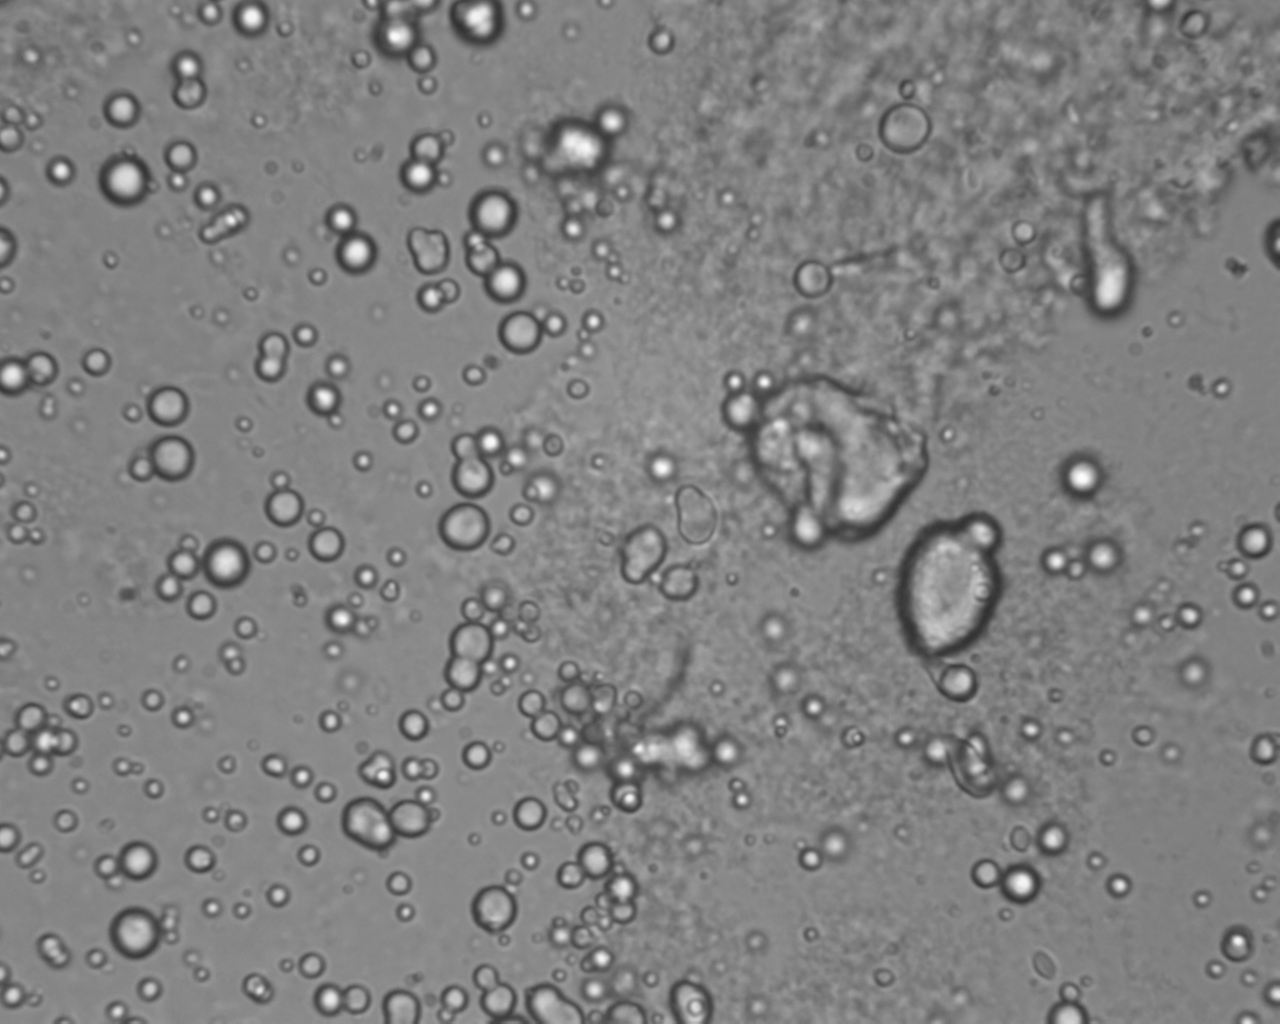
\includegraphics[width=\linewidth]{mizumoto_0.2_2.png}
          \caption{0.2v\%酢酸添加後の脂肪球2}
          \label{fig:milk0.2_2}
        \end{minipage}
      \end{figure}
      \begin{figure}[H]
        \centering
        \begin{minipage}{0.48\textwidth}
          \centering
          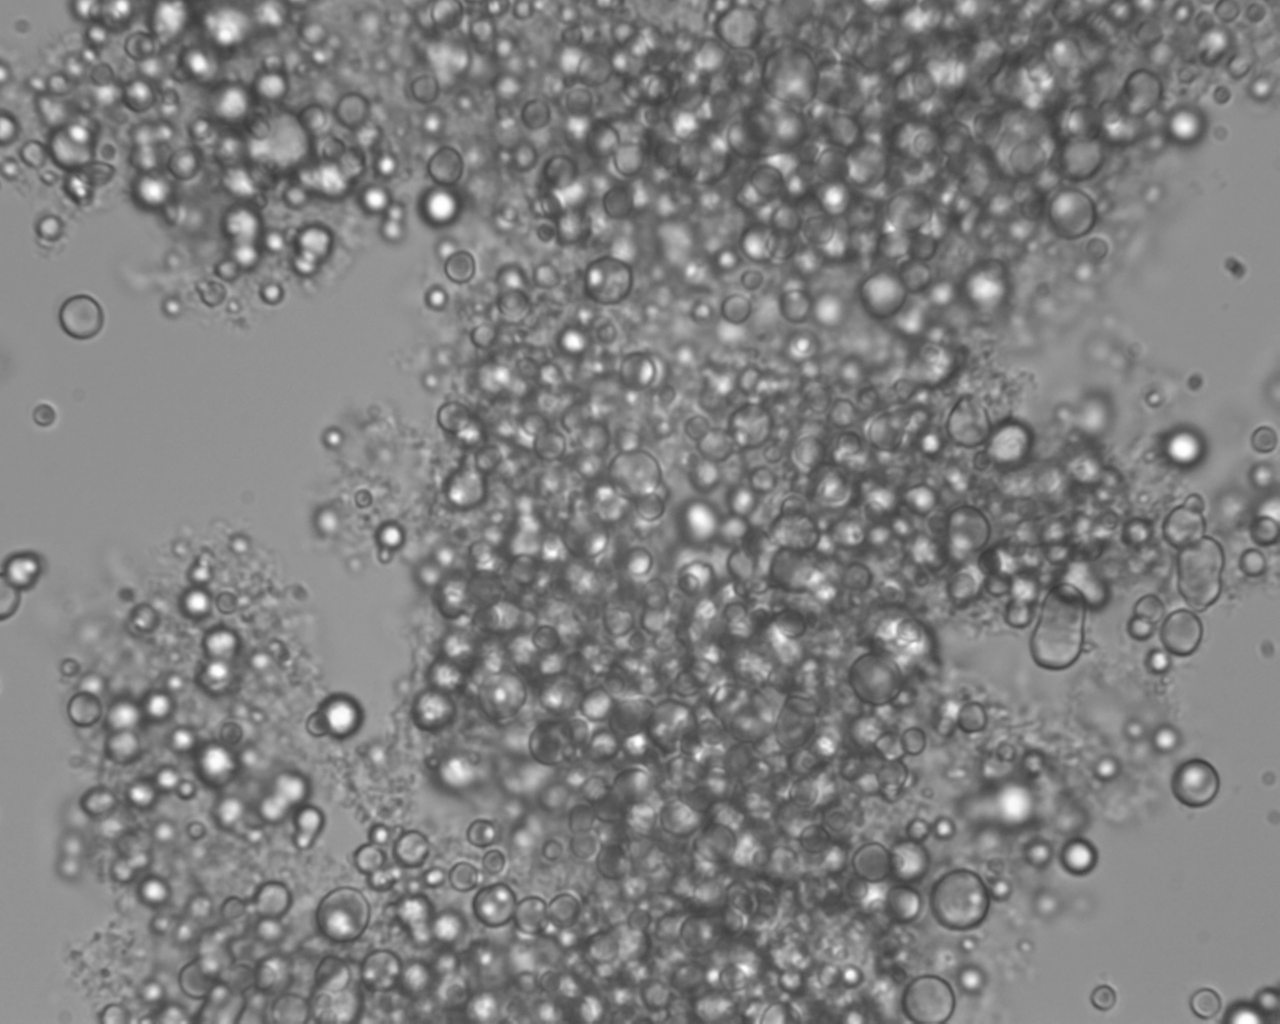
\includegraphics[width=\linewidth]{mizumoto_2_1.png}
          \caption{2v\%酢酸添加後の脂肪球1}
          \label{fig:milk2_1}
        \end{minipage}
        \hfill
        \begin{minipage}{0.48\textwidth}
          \centering
          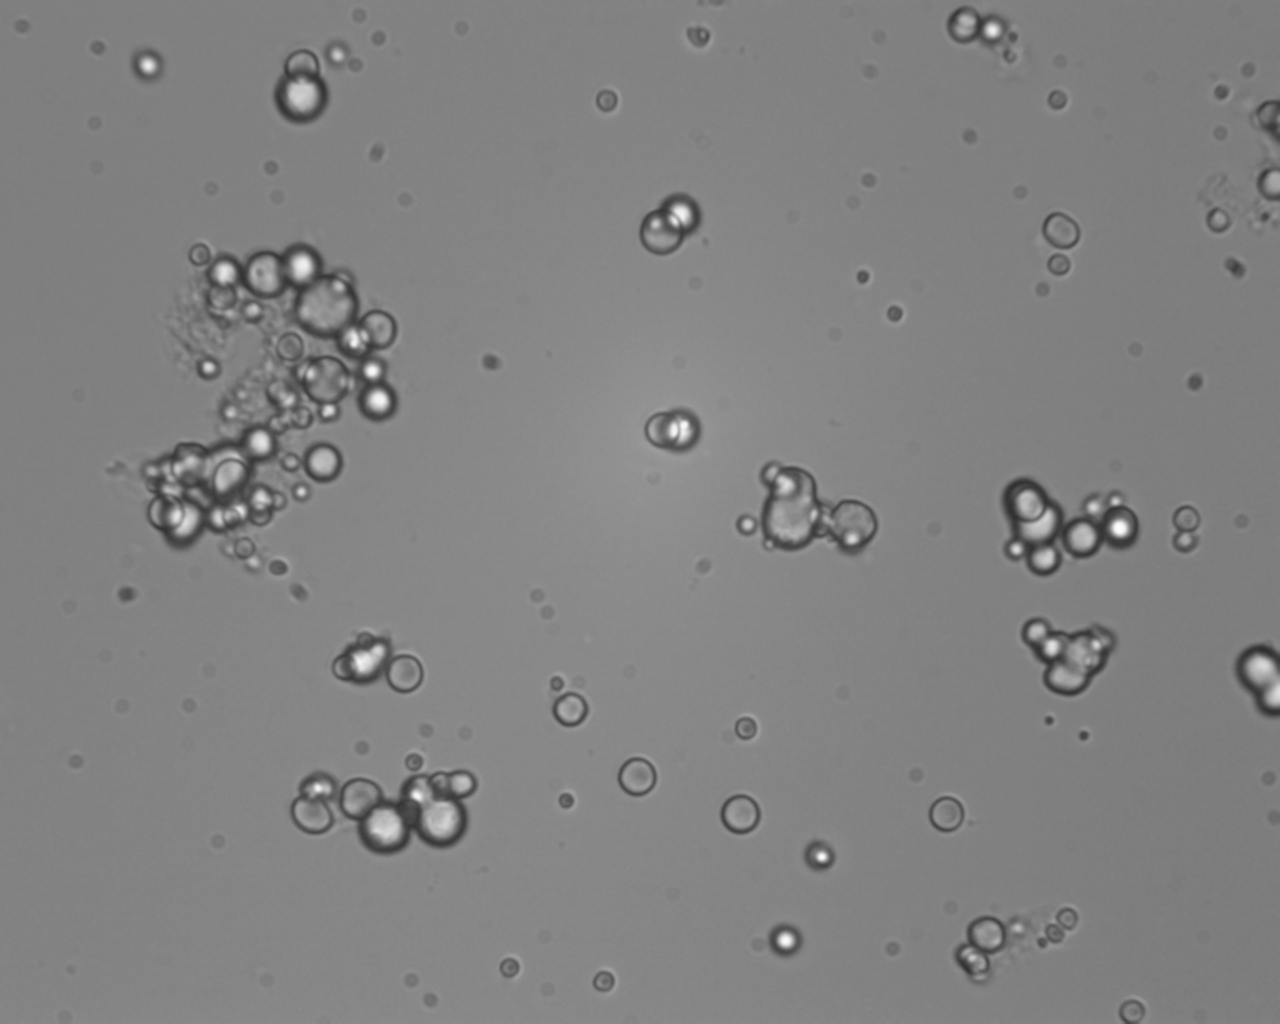
\includegraphics[width=\linewidth]{mizumoto_2_2.png}
          \caption{2v\%酢酸添加後の脂肪球2}
          \label{fig:milk2_2}
        \end{minipage}
      \end{figure}
      \begin{figure}[H]
        \centering
        \begin{minipage}{0.48\textwidth}
          \centering
          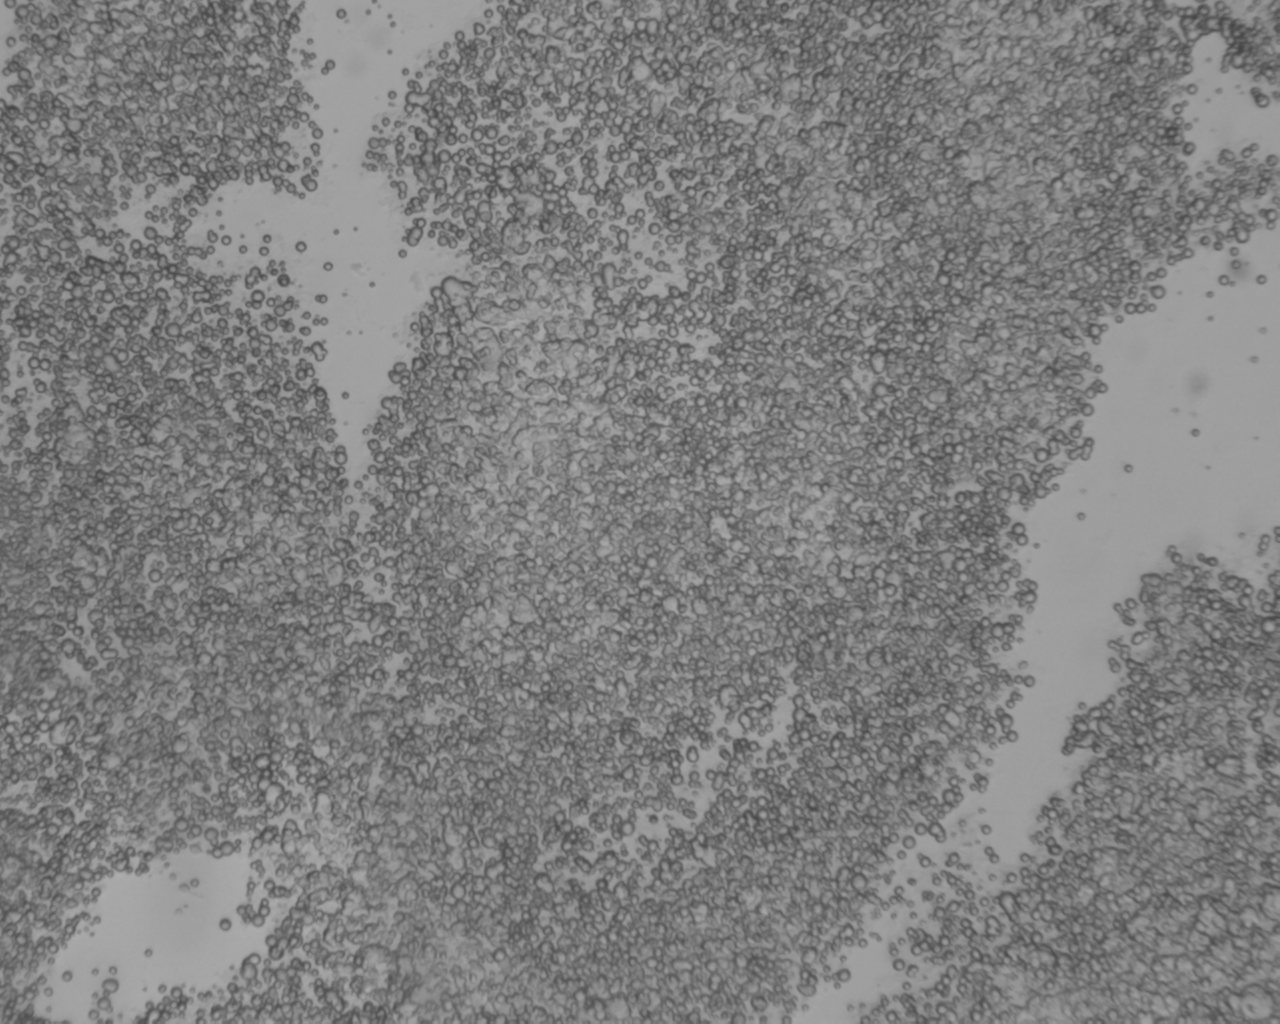
\includegraphics[width=\linewidth]{mizumoto_10_1.png}
          \caption{10v\%酢酸添加後の脂肪球1(10倍拡大)}
          \label{fig:milk10_1}
        \end{minipage}
        \hfill
        \begin{minipage}{0.48\textwidth}
          \centering
          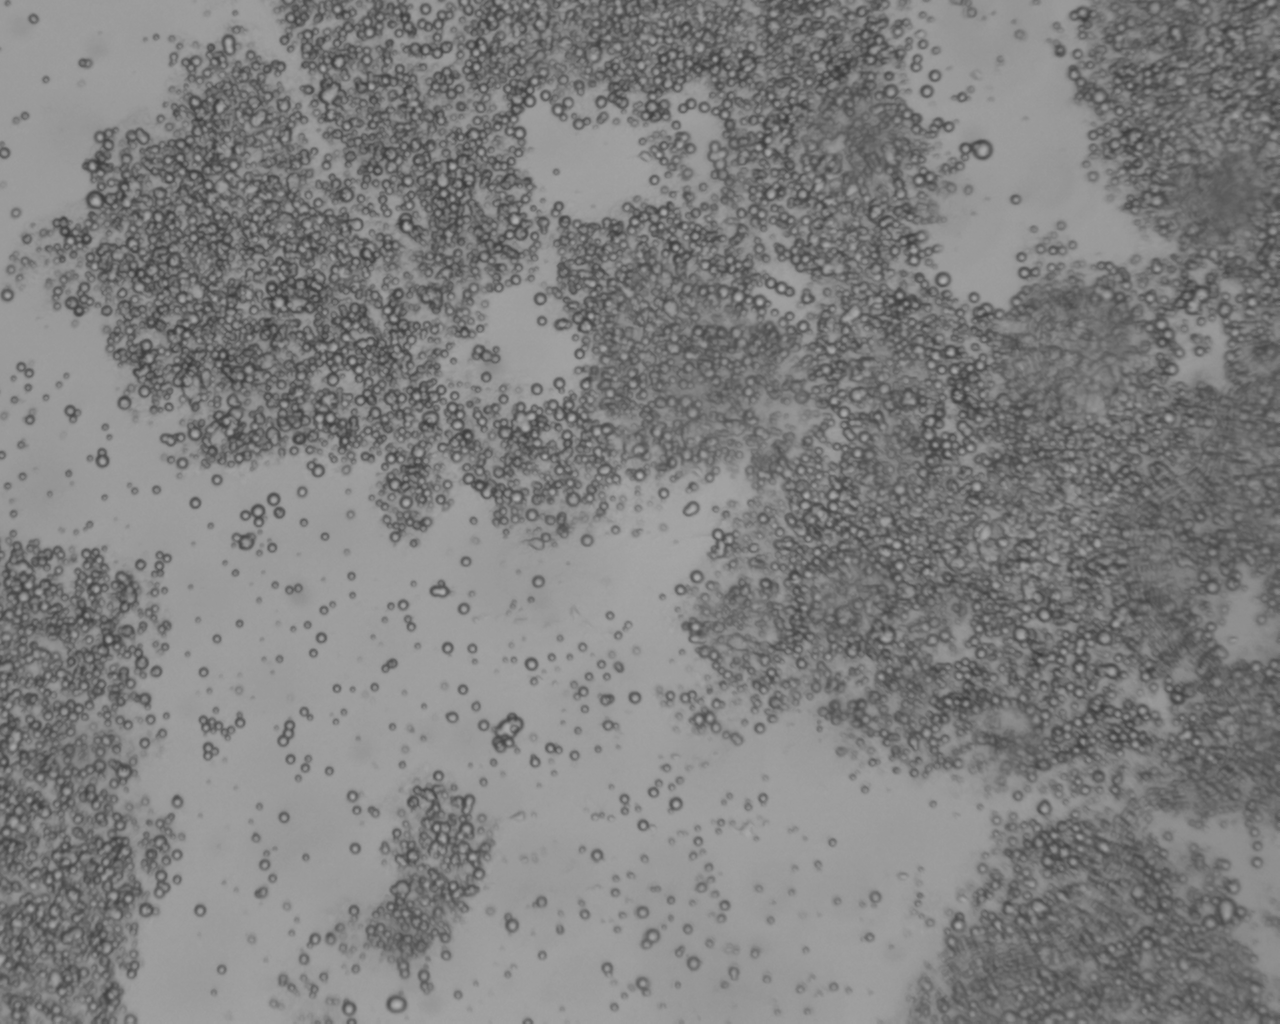
\includegraphics[width=\linewidth]{mizumoto_10_2.png}
          \caption{10v\%酢酸添加後の脂肪球2(10倍拡大)}
          \label{fig:milk10_2}
        \end{minipage}
      \end{figure}
      \begin{figure}[H]
        \centering
        \begin{minipage}{0.48\textwidth}
          \centering
          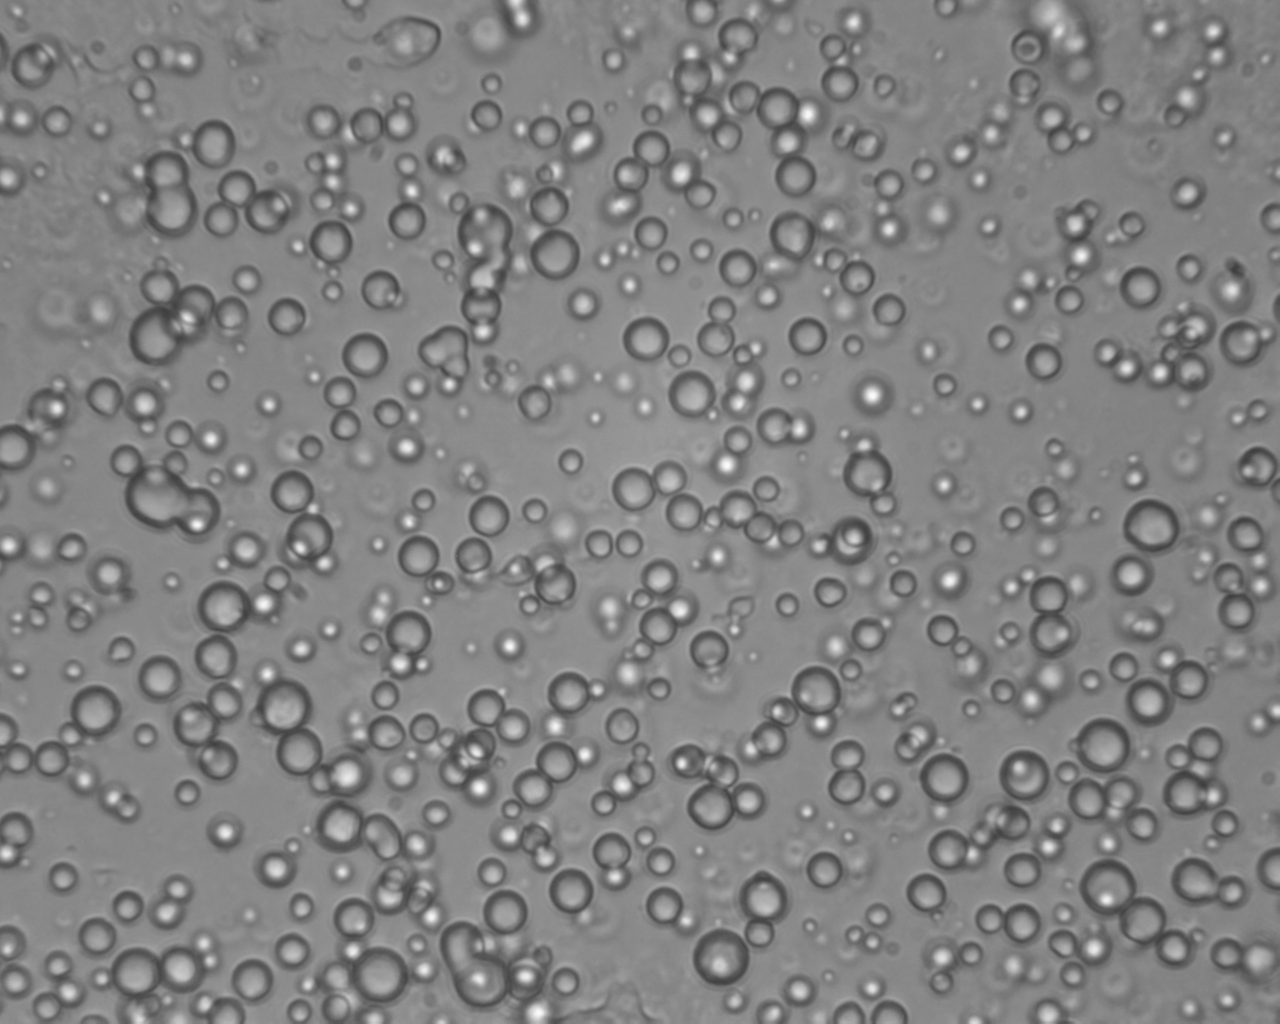
\includegraphics[width=\linewidth]{mizumoto_20_1.png}
          \caption{20v\%酢酸添加後の脂肪球1(40倍拡大)}
          \label{fig:milk20_1}
        \end{minipage}
        \hfill
        \begin{minipage}{0.48\textwidth}
          \centering
          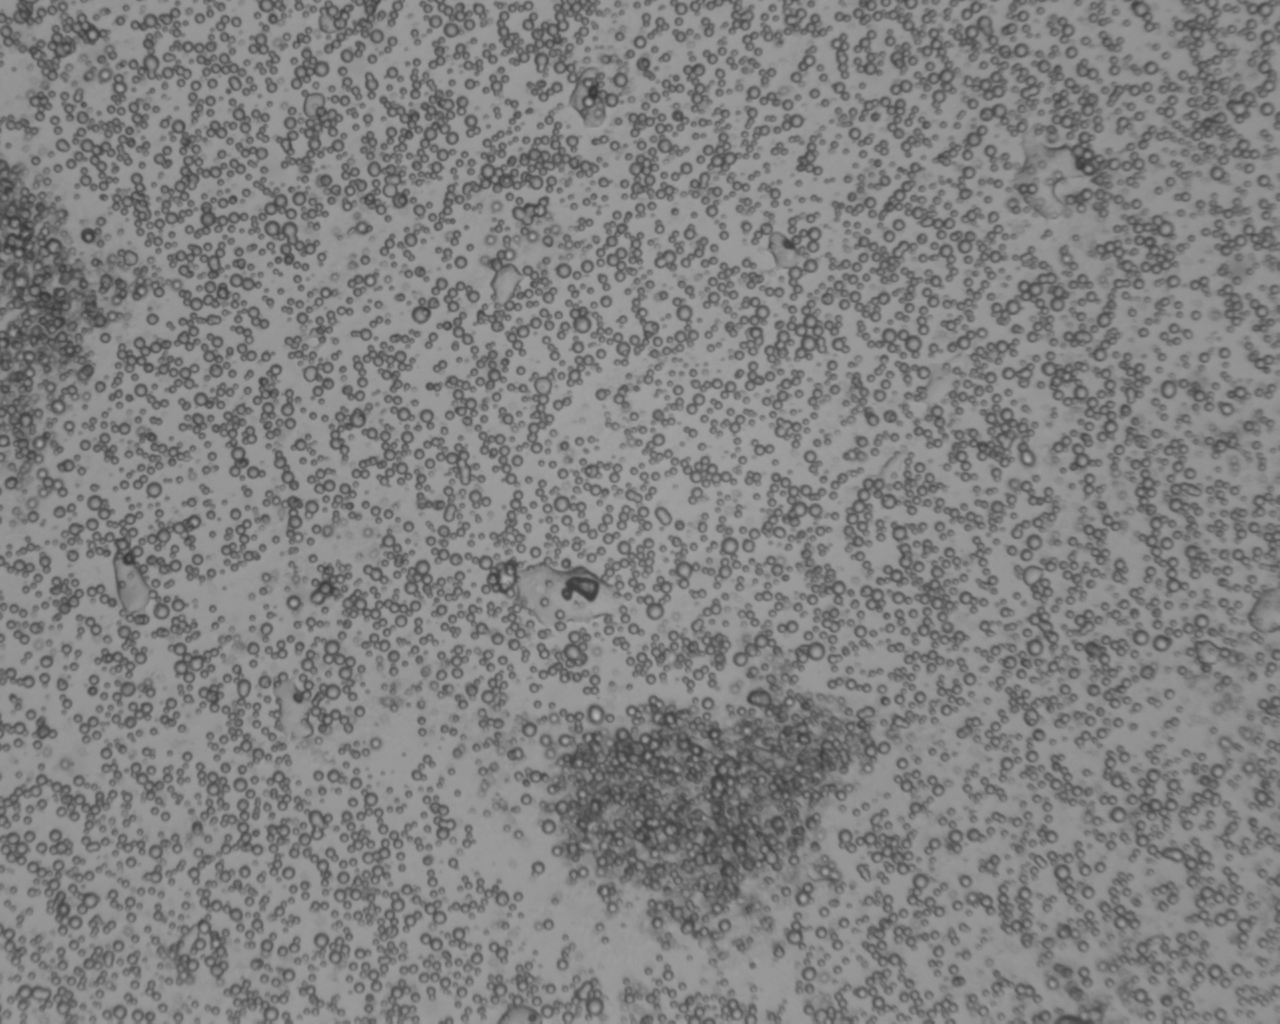
\includegraphics[width=\linewidth]{mizumoto_20_2.png}
          \caption{20v\%酢酸添加後の脂肪球2(10倍拡大)}
          \label{fig:milk20_2}
        \end{minipage}
      \end{figure}
      \begin{figure}[H]
        \centering
        \begin{minipage}{0.48\textwidth}
          \centering
          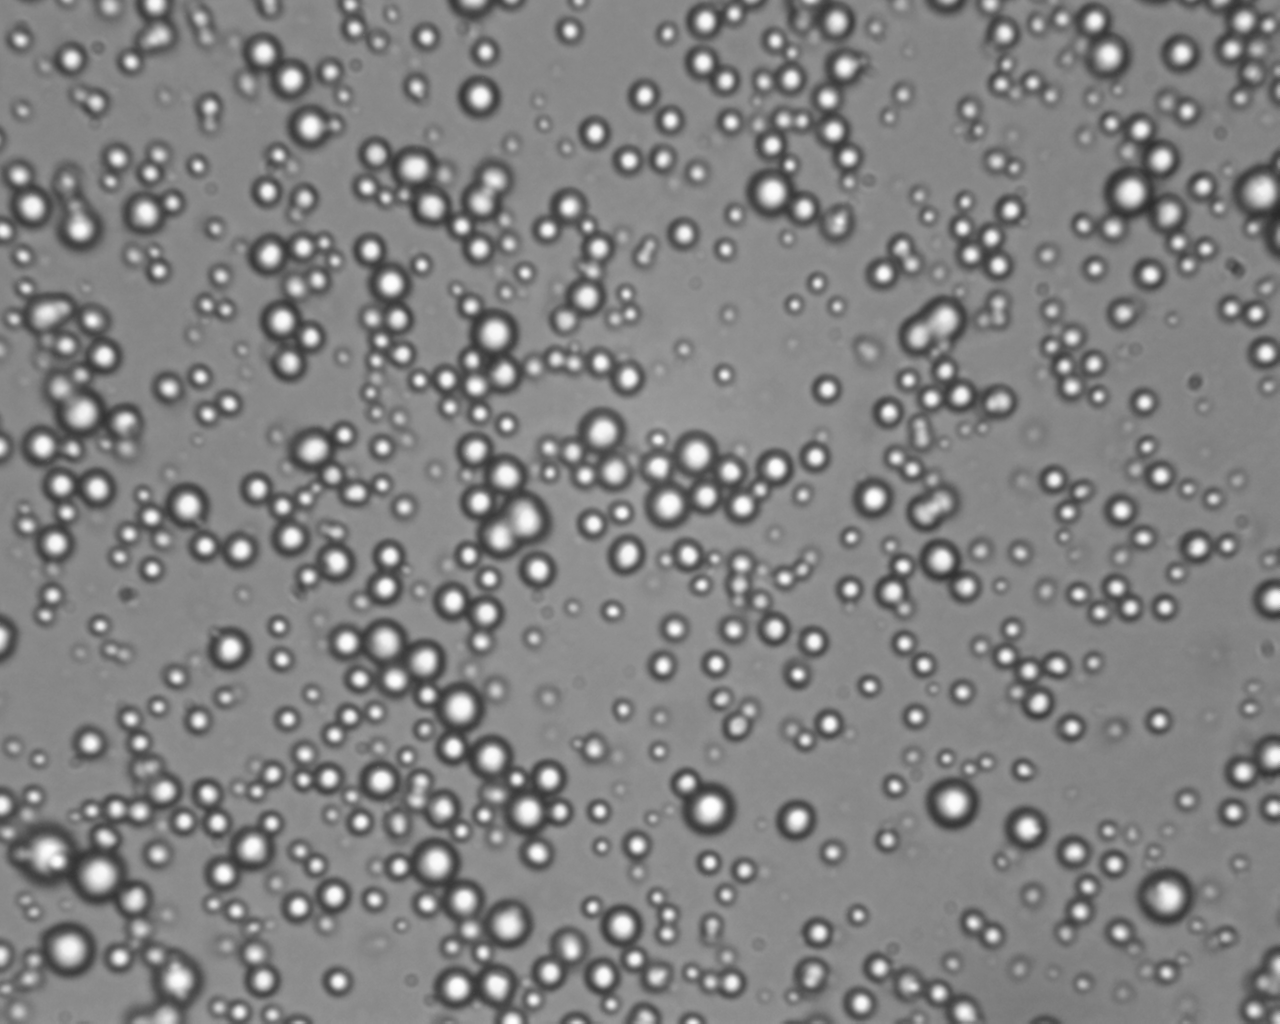
\includegraphics[width=\linewidth]{mizumoto_mizu1.png}
          \caption{水添加後の脂肪球1}
          \label{fig:aqua_1}
        \end{minipage}
        \hfill
        \begin{minipage}{0.48\textwidth}
          \centering
          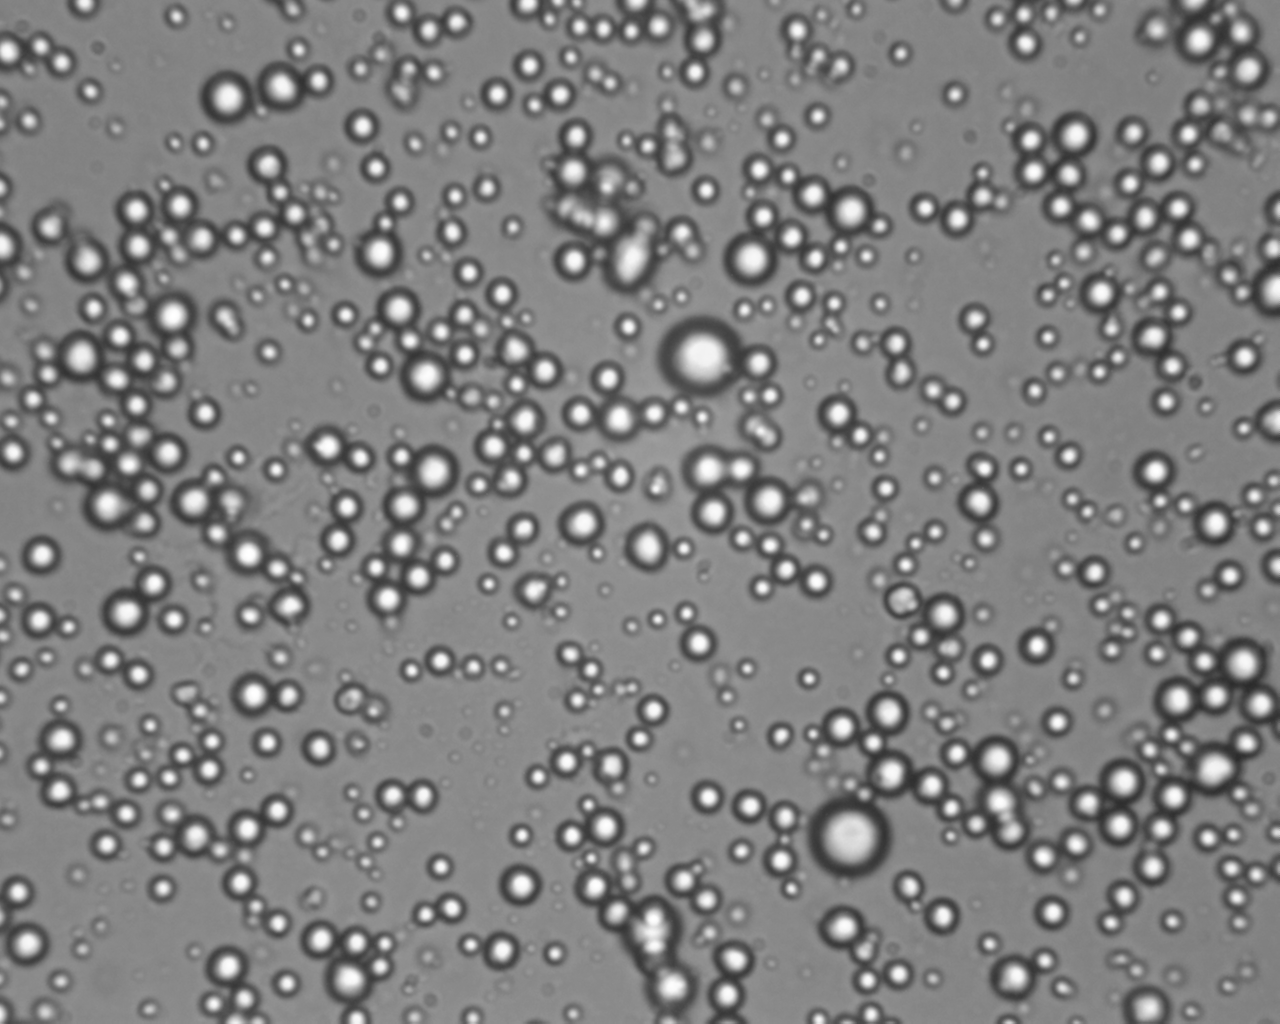
\includegraphics[width=\linewidth]{mizumoto_mizu2.png}
          \caption{水添加後の脂肪球2}
          \label{fig:aqua_2}
        \end{minipage}
      \end{figure}
      これらの画像から, 0.2v\%酢酸, 2v\%酢酸, 10v\%酢酸では, 酢酸濃度が上がるにつれて脂肪球の分散は減少し, 大きな塊となっていることがわかる. 20v\%酢酸では, 逆に分散が増加し, 水とあまり変わらない状態になっていることがわかる.
    \subsection*{課題8}
      DLVO理論では, 液体中の粒子が分散したままなのか凝集して沈殿するのかを説明する理論である.\\
      粒子間には、ファンデルワールス力による引力と, 静電気による斥力(クーロン力)が働く. この2つのどちらが優勢かによって, 粒子の挙動が決まる.\\
      \subsubsection*{分散状態}
        クーロン力がファンデルワールス力よりも大きい場合, 粒子は互いに反発しあい, 近づいても凝集しない. この状態では, 粒子は分散したままとなる.\\
      \subsubsection*{凝集状態}
        ファンデルワールス力がクーロン力よりも大きい場合, 粒子は互いに引き寄せられ, 凝集して沈殿する.\\
    \subsection*{課題9}
      カゼインは通常の牛乳中だと, 負の電荷を帯びており, クーロン力の斥力が優勢であり, 凝縮することはない. しかし, 酸によりpHが低下すると, $\mathrm{H^+}$イオンにより, カゼイン表面の負電荷が中和され, 等電点(pH=4.6)付近ではクーロン力の斥力が極端に弱まり, ファンデルワールス力が優勢となる. その結果, カゼイン同士が凝集し, 沈殿する.\\
      逆に, pHが等電点よりさらに低くなると, カゼインは正の電荷を帯びるようになり, クーロン力の斥力が再び強くなり, 粒子同士の凝集が抑制される. そのため, 酸の濃度が高い場合は, 粒子同士が分散した状態となる.\\
      このことから, 実験では酢酸濃度が高くなるにつれて脂肪球が凝縮し, 等電点を超える濃度(20v\%)では再び分散する様子が観察された.\\
    \subsubsection*{発展課題:タンパク質への影響}
      タンパク質は, pHの変化や加熱, 物理的刺激などにより変性する. 変性とは, タンパク質の立体構造が変化し, 機能を失う現象である. 観察された現象はまさしくpHによってタンパク質が変性し, 凝集する様子である.\\
  \section*{考察}
    \cref{fig:2ps_track}において, 赤色の粒子がほかの粒子と違いある地点にとどまっているように見えるのは, ほかの粒子との衝突や, 粒子が壁に近いことが原因であると考えられる.
    \cref{fig:2ps_speed}を見ても, 赤色の粒子の速度分布が他の粒子と異なり, 小さい速度の分布が大きくなっていることがわかる. \\
    また, \cref{fig:3ps_track}がブラウン運動以外の運動をしているように見えるのは, 粒子が大きくなり, ブラウン運動の影響が小さくなったからだと考えられる.\\
    また, 粒径が小さくなるにつれ, 速度分布が全体的に右にずれていることからは, 粒径が小さいほどブラウン運動の影響を受けやすいことがわかる. 
    今回, 実験で得られたアボガドロ数を文献値$N_A = 6.022 \times 10^{23} \mathrm{mol^{-1}}$と比較すると, 実験値と文献値の誤差は-18.6\%から-3.66\%となり, 誤差は大きいが, アボガドロ数を求めることができたといえる.
  \section*{まとめ}
    今回の実験では, ブラウン運動を観察し, 微粒子の統計的性質を学ぶことができた. また, 生体物質の物性や挙動についても理解を深めることができた. 
    ブラウン運動の解析手法を用いることで, アボガドロ数を求めることができ, 分子の存在を確認することができた. 
  \section*{参考文献}
    物理学総合実験生化学テキスト
\end{document}